\begin{figure}[htbp]
\centering
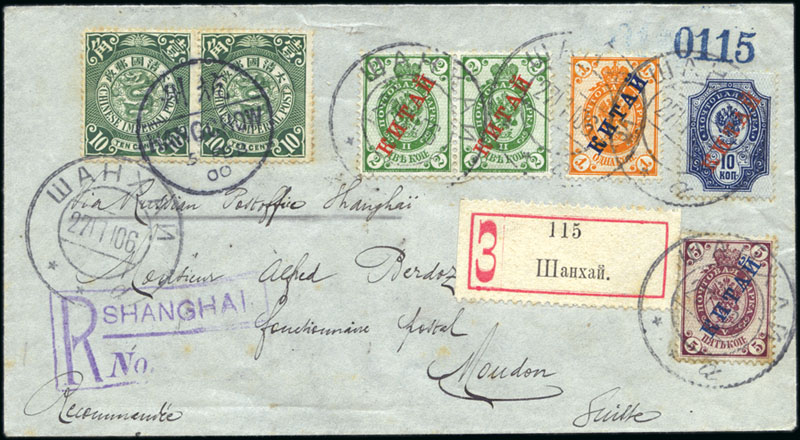
\includegraphics[width=.95\textwidth]{../russian-post-offices-in-china/10066.jpg}
\caption{
10066	SHANGHAI: 1906 Cover sent registered from Kangchow to Switzerland 
endorsed "via Russian Post Office Shanghai," with China 10c Dragon pair 
tied by Kangchow bilingual cds, sent to Shanghai where it was passed to 
the Russian P.O. and franked with "KITAI" 1k, 2k (2), 5k and 10k tied by 
Shanghai 27.1.06 cds (T\&S type 3), reg'd label in Cyrillic and boxed 'R' 
reg'n hs adjacent, Hong Kong and Moudon bs, attractive mixed country franking
\euro 800.00 
}  
\end{figure} 

\begin{figure}[htbp]
\centering
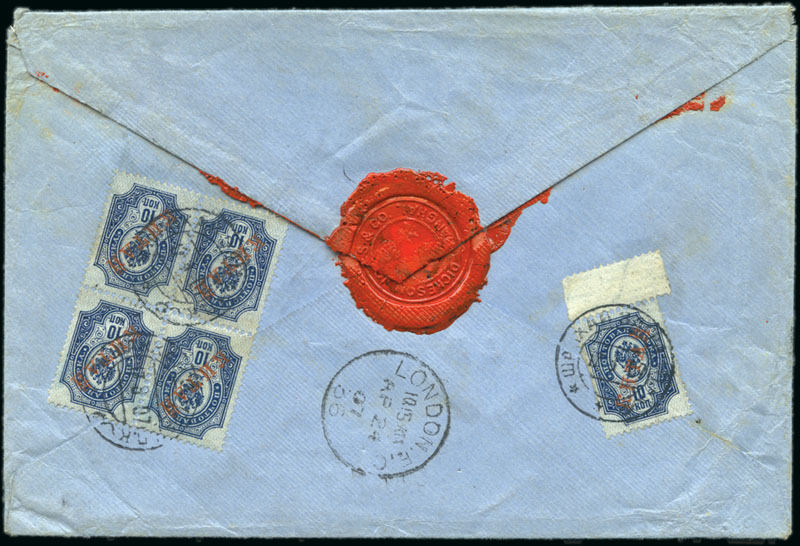
\includegraphics[width=.95\textwidth]{../russian-post-offices-in-china/10067.jpg}
\caption{
10067 SHANGHAI: 1907 Cover to England "via Siberia" franked on the 
reverse with "KITAI" 10k in block of four and single paying 5 times 
the 10k foreign letter rate, tied by Shanghai 17.3.07 cds (T\&S type 5B), 
London arrival, a scarce rate.
\euro 200.00
}  
\end{figure}

\begin{figure}[htbp]
\centering
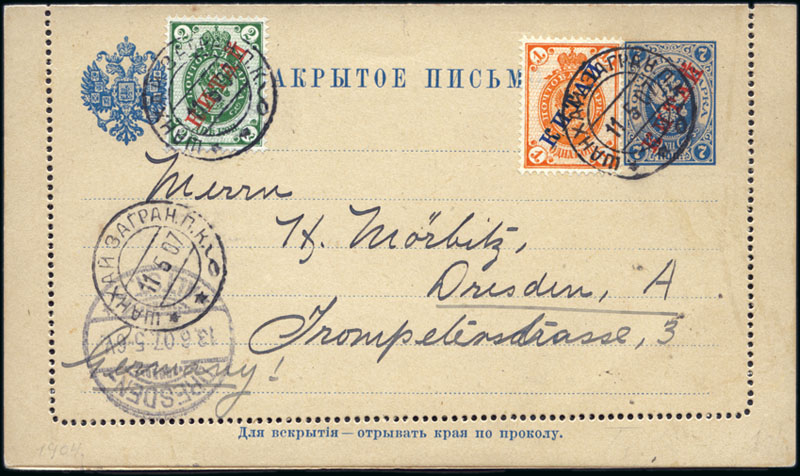
\includegraphics[width=.95\textwidth]{../russian-post-offices-in-china/10068.jpg}
\caption{
10068	SHANGHAI: "KITAI" 7k letter card to Germany, uprated with 
"KITAI" 1k and 2k paying the 10k foreign letter rate, all cancelled by 
Shanghai 11.5.07 cds (T\&S type 5B), Dresden arrival, very fine.
\euro200.00 
}  
\end{figure} 

\begin{figure}[htbp]
\centering
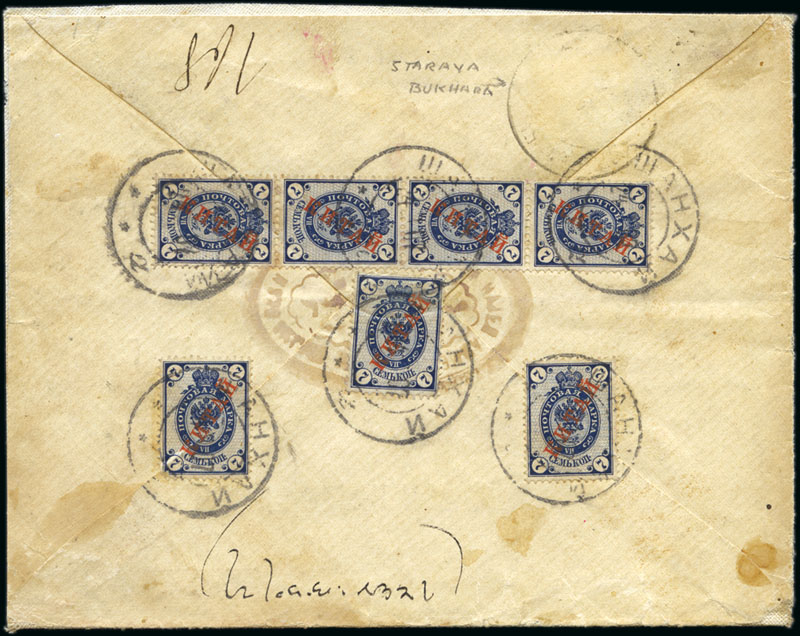
\includegraphics[width=.95\textwidth]{../russian-post-offices-in-china/10069.jpg}
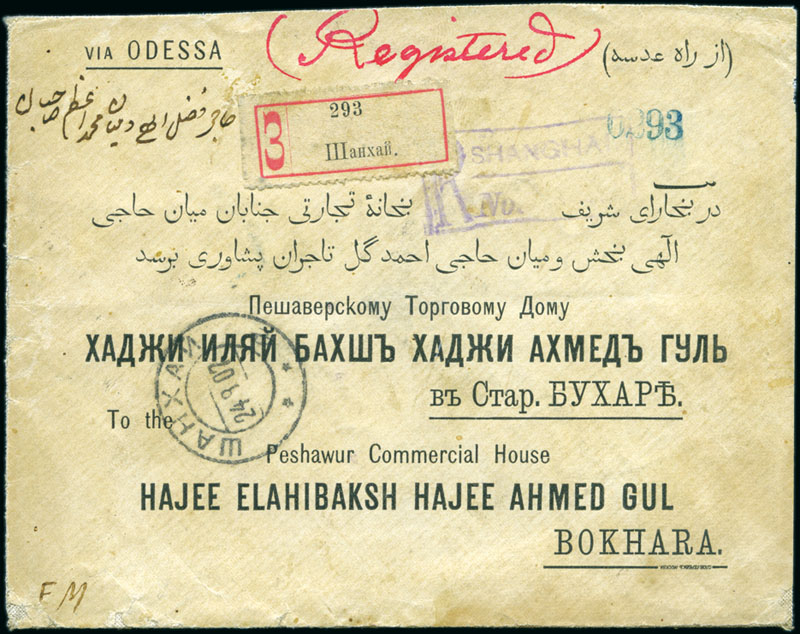
\includegraphics[width=.95\textwidth]{../russian-post-offices-in-china/10069-1.jpg}
\caption{
10069		ZoomSHANGHAI: 1907 Cover registered to Staraya, Bukhara 
(in modern day Uzbekistan), franked on the reverse with seven "KITAI" 
7k paying six times the 7k internal rate plus reg'n fee, tied by Shanghai 
24.8.07 cds (T\&S type 3), with registration label in Cyrillic and boxed 
reg'n hs in English adjacent, opened on three sides, a scarce rate.
\euro 200.00
}  
\end{figure}

\begin{figure}[htbp]
\centering
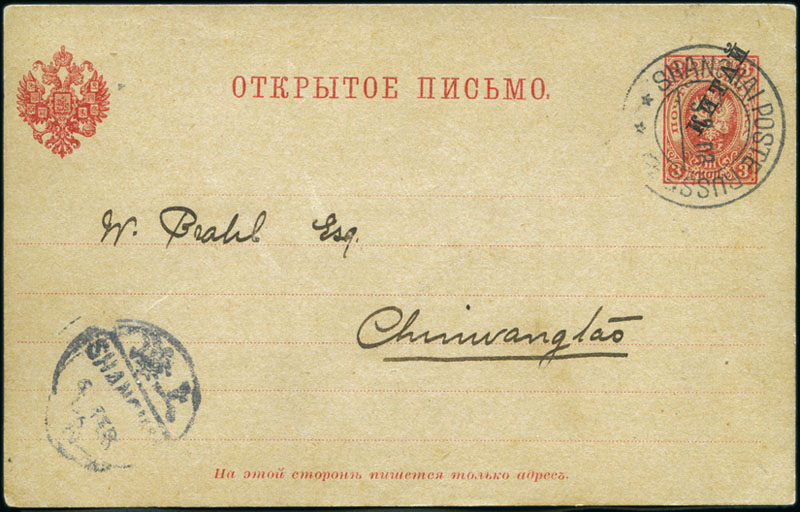
\includegraphics[width=.95\textwidth]{../russian-post-offices-in-china/10070.jpg}
\caption{
10070	SHANGHAI: 1908 3k 'Kitai' stationery card (overprint misplaced) 
addressed
to Chinwangtao, China, neatly cancelled by SHANGHAI POSTE RUSSE cds (Subtype 6A),
with un cancelled CIP 1c on reverse with interesting inscription 
"They would not
accept postcards for China at the British \& the Russian PO so I 
am trying this way",
very fine, unusual \& scarce

Note: The foreign PO's in China existed for transmission of mail abroad, 
since China was not a member of the UPU and its stamps had no validity 
for postage outside the country.
\euro 300.00
}  
\end{figure}
  